
\documentclass[twocolumn]{article}
\usepackage{hyperref}
\usepackage{enumitem}
\usepackage{graphicx}
\usepackage{amsmath}
\usepackage{mathpazo}
\usepackage{xcolor}
\usepackage{float}
\usepackage{listings}
\lstset{
  basicstyle=\ttfamily\small,
  breaklines=true,
  columns=fullflexible,
  frame=single,
  showspaces=false,
  showtabs=false,
  keepspaces=false
}

% \usepackage{multicol}
\usepackage[a4paper,
            bindingoffset=0.2in,
            left=0.5in,
            right=0.5in,
            top=0.5in,
            bottom=0.5in,
            footskip=.25in]{geometry}


\begin{document}
\title{MS Technical Paper: \\ Placement Algorithms for Heterogenous FPGAs}
\author{Brian B Cheng \\ Rutgers University Department of Electrical and Computer Engineering}


\date{}
\maketitle

\section{Keywords}
\begin{itemize}
    \item FPGA, EDA, Placement, Simulated Annealing, Optimization, RapidWright
\end{itemize}


\section{Abstract}
    fdsafdsafdsa. \\ 
    fdsafdsafdsa. \\ 
    fdsafdsafdsa. \\ 
    fdsafdsafdsa. \\ 
    fdsafdsafdsa. \\ 
    fdsafdsafdsa. \\ 
    fdsafdsafdsa. \\ 
    fdsafdsafdsa. \\ 
    fdsafdsafdsa. \\ 
    fdsafdsafdsa. \\ 
    fdsafdsafdsa. \\ 
    fdsafdsafdsa. \\ 
    fdsafdsafdsa. \\ 

\section{Introduction}

    Field-Programmable Gate Arrays (FPGAs) have witnessed rapid growth in capacity and versatility, driving significant advances in computer-aided design (CAD) and electronic design automation (EDA) methodologies. 
    Since the early-to-mid 2000s, the stagnation of single-processor performance relative to the rapid increase in integrated circuit sizes has led to a design productivity gap, where the computational effort for designing complex chips continues to rise. 
    FPGA CAD flows mainly encompass synthesis, placement, and routing; all of which are HP-hard problems, of which placement is one of the most time-consuming processes. 
    Inefficienct placement strategy not only extends design times from hours to days, thereby elevating cost and reducing engineering productivity, but also limits the broader adoption of FPGAs by software engineers who expect compile times akin to those of conventional software compilers like {\tt gcc}. 

    For these reasons, FPGA placement remains a critical research effort even today. 
    In this paper, we study and implement established placement methods. 
    To do this, we use the RapidWright API, which is a semi-open-source research effort from AMD/Xilinx that enables custom solutions to FPGA design implementations and design tools that are not offered by their industry-standard FPGA environment, Vivado. 
    We implement multiple variations of simulated annealing placers for Xilinx's 7-series FPGAs, with an emphasis on minimizing total wirelength while mitigating runtime. 
    Our implementation is organized into three consecutive substages. 
    The \textbf{prepacking} stage involves traversing a raw EDIF netlist to identify recurring cell patterns—such as CARRY chains, DSP cascades, and LUT-FF pairs—that are critical for efficient mapping and legalization. 
    In the subsequent \textbf{packing} stage, these identified patterns, along with any remaining loose cells, are consolidated into SiteInst objects that encapsulate the FPGA’s discrete resource constraints and architectural nuances. 
    Finally, the \textbf{placement} stage employs a simulated annealing (SA) algorithm to optimally assign SiteInst objects to physical sites, aiming to minimize total wirelength while adhering to the constraints of the 7-series architecture. 

    Simulated annealing iteratively swaps placement objects guided by a cost function that decides which swaps should be accepted or rejected. 
    Hill climbing is permitted by occasionally accepting moves that increase cost, in hope that such swaps may later lead to a better final solution. 
    SA remains a popular approach in FPGA placement research due to its simplicity and robustness in handling the discrete architectural constraints of FPGA devices. 
    While SA yields surprisingly good results given relatively simple rules, it is ultimately a heuristic and stochastic approach that explores the vast placement space by making random moves. 
    Most of these moves will be rejected, meaning that SA must run many iterations, usually hundreds to thousands, to arrive at a desirable solution. 

    In the ASIC domain, where placers must handle designs with millions of cells, the SA approach has largely been abandoned in favor of analytical techniques, owing to SA's runtime and poor scalability. 
    Modern FPGA placers have also followed suit, as new legalization strategies allow FPGA placers to leverage traditionally ASIC placement algorithms and adapt them to the discrete constraints of FPGA architectures. 
    While this paper does not present a working analytical placer, it will explore ways to build upon our existing infrastructure (prepacker and packer) to replace SA with AP. 

\section{A Brief History on FPGA Architecture}

    \begin{figure}
        \centering
        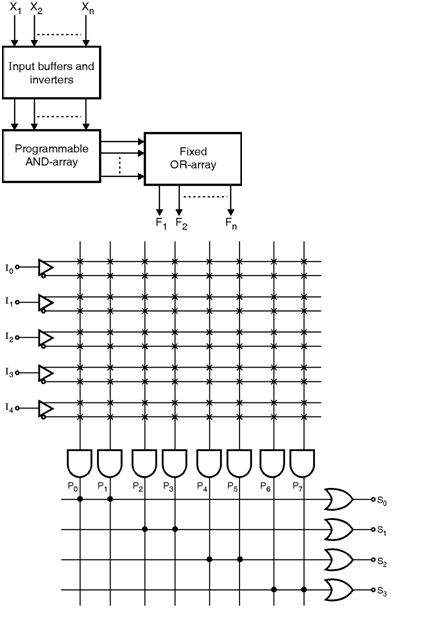
\includegraphics[width=8.0cm]{figures/pal_2.png}
        \caption{PAL architecture with 5 inputs, 8 programmable AND gates and 4 fixed OR gates}
        \label{fig:pla}
        % https://www.electronics-tutorial.net/Programmable-Logic-Device-Architectures/Programmable-Logic-Devices/Programmable-Array-Logic-PAL/
        % https://www.naukri.com/code360/library/difference-between-pla-and-pal 
    \end{figure}

    Before any work can begin on an FPGA placer, it is necessary to understand both the objects being placed and the medium in which they are placed.

    Here we will briefly outline the evolution of configurable logic architecture as well as the FPGA design flow. 
    However, readers who are already familiar with basic FPGA architecture and design flow may skip to the next section on Xilinx 7-Series Architecture. 
    Configurable logic devices have undergone significant evolution over the past four decades. 
    The journey began with the Programmable Logic Array (PLA) in the early 1970s. 
    The PLA implemented output logic using a programmable-OR and programmable-AND plane that formed a sum-of-products equation for each output through programmable fuses. 
    Around the same time, the Programmable Array Logic (PAL) was introduced. 
    The PAL simplified the PLA by fixing the OR gates, resulting in a fixed-OR, programmable-AND design, which sacrificed some logic flexibility to simplify its manufacture. 
    Figure \ref{fig:pla} shows one such PLA architecture. 

    \begin{figure}
        \centering
        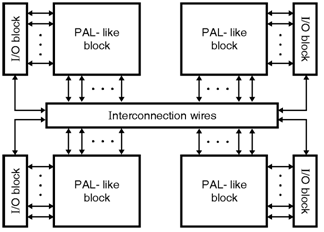
\includegraphics[width=8.0cm]{figures/cpld.png}
        \caption{CPLD architecture with 4 CLBs (PAL-like blocks)}
        \label{fig:cpld}
        % https://www.electronics-tutorial.net/Programmable-Logic-Device-Architectures/CPLD/Complex-Programmable-Logic-Device-CPLDs/
    \end{figure}

    Later in the same decade came the Complex Programmable Logic Device (CPLD), which took the form of an array of Configurable Logic Blocks (CLBs). 
    These CLBs were typically modified PAL blocks that included the PAL itself along with macrocells such as flip-flops, multiplexers, and tri-state buffers. 
    The CPLD functioned as an array of PALs connected by a central programmable switch matrix and could be programmed using a hardware description language (HDL) like VHDL. 
    Figure \ref{fig:cpld} shows one such CPLD architecture. 

    \begin{figure}
        \centering
        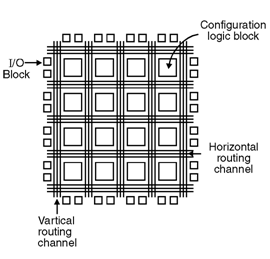
\includegraphics[width=8.0cm]{figures/homogenous_fpga.png}
        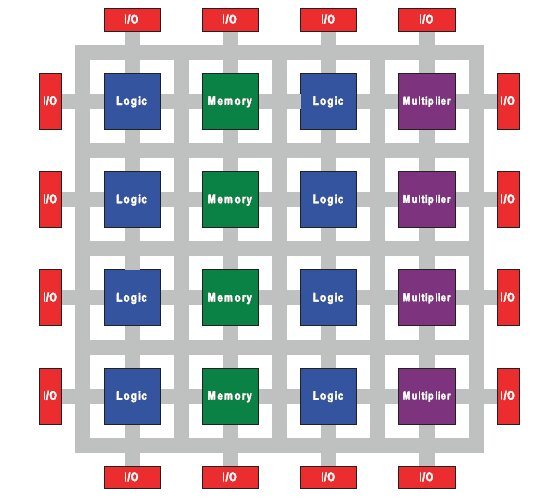
\includegraphics[width=8.0cm]{figures/heterogenous_fpga_3.jpg}
        \caption{
            \textbf{Top}: A homogeneous island-style FPGA architecture with 16 CLBs in a grid. 
            \textbf{Bottom}: A heterogeneous island-style FPGA with a mix of CLBs and macrocells.
        }
        \label{fig:fpga}
        % https://www.electronics-tutorial.net/Programmable-Logic-Device-Architectures/FPGA/Field-programmable-gate-array-FPGA/
        % https://www.electronics-tutorial.net/Programmable-Logic-Device-Architectures/FPGA/Field-programmable-gate-array-FPGA/
    \end{figure}

    The mid-1980s saw the introduction of the homogeneous FPGA, which was built as a grid of CLBs. 
    Rather than using a central programmable switch matrix as in CPLDs, FPGAs adopted an island style architecture in which each CLB is surrounded on all sides by programmable routing resources, as shown in Figure \ref{fig:homogenous_fpga}. 
    The first commercially viable FPGA, produced by Xilinx in 1984, featured 16 CLBs arranged in a 4x4 grid. 
    As FPGA technology advanced, CLBs were redesigned to use lookup tables (LUTs) instead of PAL arrays for greater logic density. 
    The capacity of an FPGA was often measured by how many logical elements or CLBs it offered, which grew from hundreds to thousands and now to hundreds of thousands of CLBs.


    This brings us to modern day FPGA architectures.
    To meet the needs of increasingly complex designs, FPGA vendors introduced heterogeneous FPGAs. 
    In these devices, hard macros such as Block RAM (BRAM) and Digital Signal Processing (DSP) slices are integrated into the programmable logic fabric along with CLBs, like shown in Figure \ref{fig:fpga}. 
    This design enables the direct instantiation of common subsystems like memories and multipliers, without having to recreate them from scratch using CLBs. 
    Major vendors such as Xilinx and Altera now employ heterogeneous island-style architectures in their devices. 
    As designs become increasingly large and complex, FPGAs become increasingly heterogenous by incorporating a wider variety of hard macros into the fabric.

\section{The FPGA Design Flow and Toolchain}
    
    \begin{figure}
        \centering
        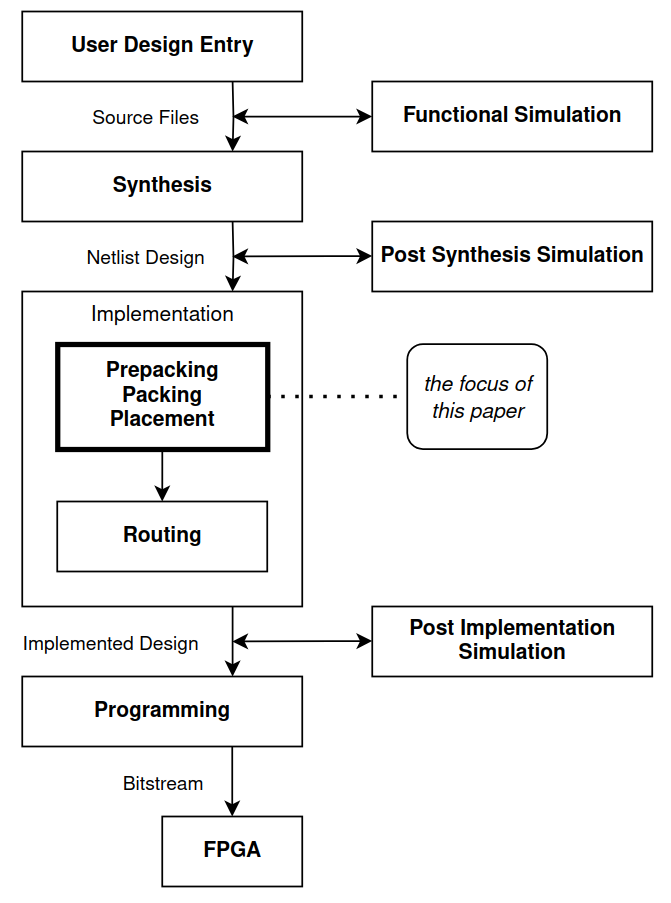
\includegraphics[width=7.0cm]{figures/design_flow.png}
        \caption{A typical FPGA design and verification workflow}
        \label{fig:design_flow}
    \end{figure}

    Figure \ref{fig:design_flow} shows a typical FPGA design and verification workflow.
    The FPGA design flow takes a high-level digital design written in an HDL and generates a configuration file that programs the physical FPGA. 

    The process begins with \textbf{design entry}, where an engineer describes the functionality of their circuit using a hardware description language (HDL) such as Verilog or VHDL. This description abstracts away details of the physical hardware while defining the logic and behavior of the design.

    Next, the \textbf{synthesis} tool interprets the HDL code and generates a netlist that represents the design in terms of primitive cells, such as lookup tables (LUTs) and flip flops. 
    This is the result of the synthesis tool parsing the raw Verilog source files, inferring logical behavior, and instantiating primitive cells to emulate the desired logical behavior. 
    The final stage is often referred to as "technology mapping", as the primitive cells are specific to the FPGA architecture and consequently the FPGA manufacturer. 

    After synthesis, the \textbf{placement} tool assigns each logic element in the netlist a specific location within the FPGA’s fabric. 
    Depending on the placement strategy, this stage can include substages of prepacking, packing, global placement, legalization, and detailed placement. 
    Our placer will only involve prepacking, packing, and detailed placement for simplicity. 
    The objective is to place the logical cell instances of the netlist onto physical BELs on the device in a way that minimizes delay, satisfies design constraints, and simplifies routing. 

    Following placement, the \textbf{routing} tool connects the placed elements by assigning physical wiring resources to the nets in the netlist. 
    The router determines their paths through the programmable interconnect network while attempting to meet timing and performance constraints.

    Placement and routing are generally referred to together as the \textbf{implementation} stage, as both stages are interdependent and must adhere to the constraints of the same device. 
    State of the art (SOTA) tools will perform routing-aware placement for greater optimization. 

    The final stage is the \textbf{bitstream} generation, where a vendor-specific programming tool produces a configuration file or bitstream that programs the physical FPGA device. 
    The bitstream specifies the state of every configurable element—logic blocks, routing switches, and hard macros—ensuring the FPGA implements the user's design. 


    Parallel to this entire design flow are simulators for which the user can write testbenches to verify their design at different stages of implementation.
    Xilinx's Vivado, for example, provides functional simulation, post-implementation simulation, and post-implementation timing simulation.

    This integrated toolchain, whether provided by FPGA vendors or open source communities, facilitates the transformation from an abstract HDL description to a functioning hardware configuration.


\section{Xilinx 7-Series Architecture}

    \begin{figure*}[t]
        \centering
        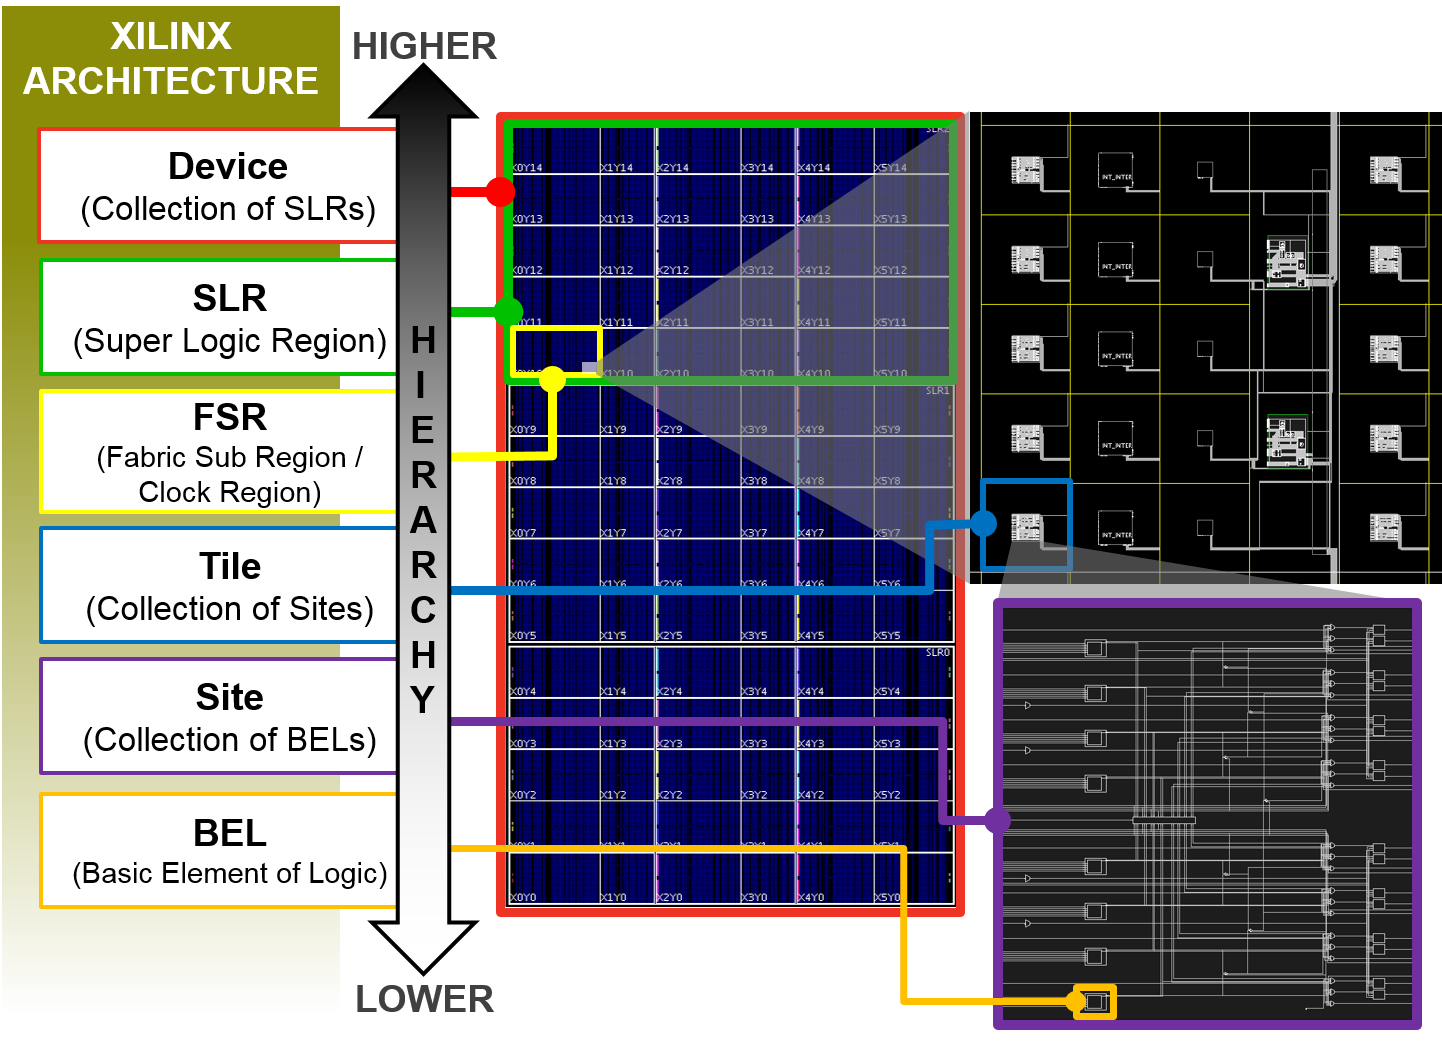
\includegraphics[width=12.0cm]{figures/hierarchy.png}
        \caption{Architecture Hierarchy of a Xilinx FPGA (Ultrascale)}
        \label{fig:hierarchy}
    \end{figure*}

    Xilinx introduced the 7-Series architecture in 2010 which followed the heterogeneous island-style architecture described previously. 
    Then in 2013 Xilinx unveiled Ultrascale architecture which also followed the heterogenous island-style design but made several improvements over the 7-Series architecture.
    Although the latest FPGAs follow the Ultrascale architecture, this paper focuses on the 7-Series FPGAs due to their greater accessibility for beginner users and compatibility with open source tooling.


    Figure~\ref{fig:hierarchy} illustrates the architectural hierarchy of an Ultrascale Xilinx FPGA. 
    The architecture hierarchy is the same for the 7-Series devices. 
    At its most basic level, an FPGA is a vast physical array of replicated atomic components known as Basic Elements of Logic (BELs). 
    These BELs, which include LUTs, FFs, BRAMs, DSPs, and programmable interconnects, form the fundamental building blocks for custom digital circuit implementations on FPGAs. 

    The Xilinx architectural hierarchy organizes these BELs into increasingly abstract structures. 
    \textbf{BELs} are packaged into \textbf{Sites}, which are then embedded into \textbf{Tiles}, which are subsequently consolidated into \textbf{Clock Regions}. 
    In high-end Xilinx devices, Clock Regions may be further consolidated into \textbf{Super Logic Regions} (SLRs). 
    However, for the scope of this paper, we focus on Xilinx devices that have only a single SLR. 


\section{RapidWright API}
    We use the RapidWright API to implement a custom placer for Xilinx 7-Series FPGAs.
    RapidWright is an open source Java framework that enables netlist implementation manipulation for modern Xilinx FPGAs. 

    \begin{figure}[]
        \centering
        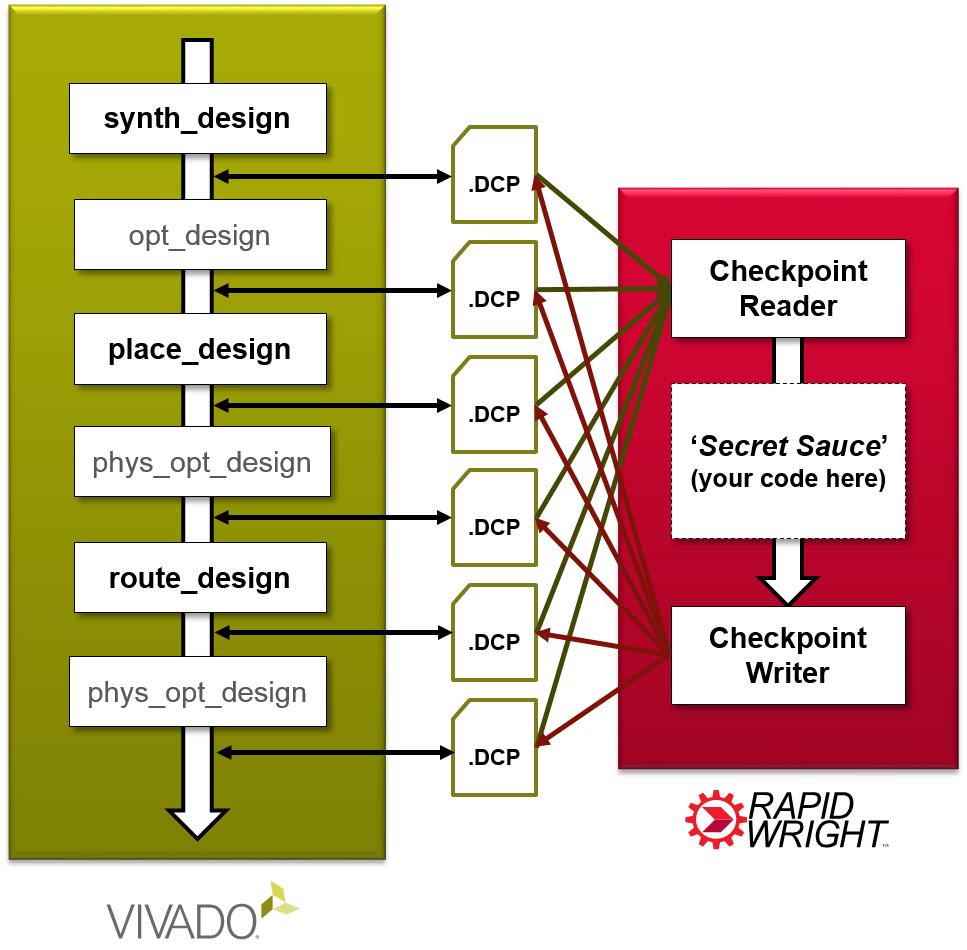
\includegraphics[width=8.0cm]{figures/vivado_dcps.png}
        \caption{Showing how RapidWright can take a design checkpoint from any stage of the design flow, allow user customization, and reintegrate it back into the design flow.}
        \label{fig:vivado_dcps}
    \end{figure}

    \begin{figure}[]
        \centering
        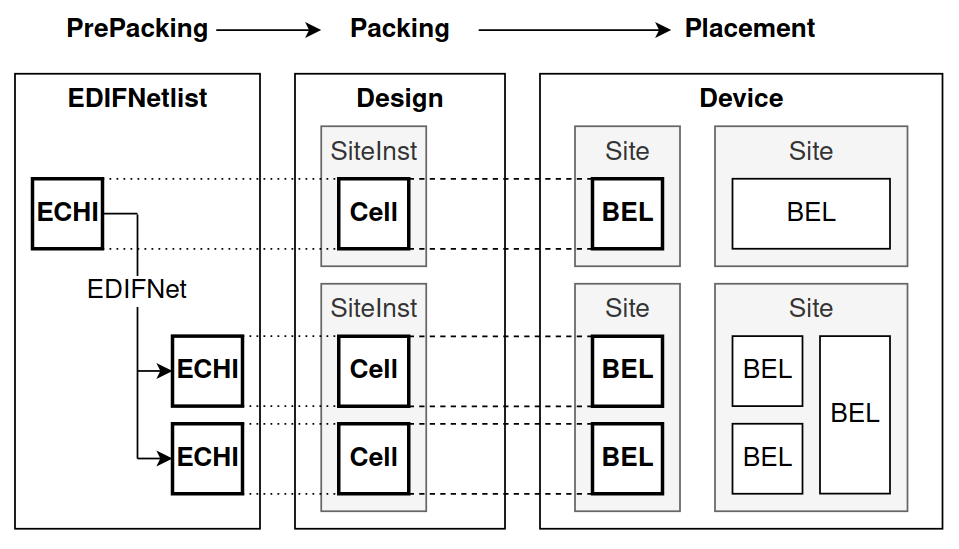
\includegraphics[width=8.5cm]{figures/edif_design_device.png}
        \caption{The placement flow illustrating PrePacking into Packing into Placement for a logical netlist with 3 EDIF cells. EHCI is short for EDIFHierCellInst.}
        \label{fig:edif_design_device}
    \end{figure}

    Figure \ref{fig:vivado_dcps} shows how the API allows us to take design checkpoints in the form of .dcp files generated at any stage of the design flow, allow the user to make custom optimizations, and reintegrate it back into the design flow. 
    This allows the user to substitute any stage in the default FPGA design flow offered by Vivado with a custom user-defined process to meet complex design constraints. 
    There are three packages of objects that are most relevant to building our placer: the \textbf{edif} package, \textbf{design} package, and \textbf{device} package. 
    Figure \ref{fig:edif_objects} shows the EDIF netlist objects and device routing objects as shown in the Vivado netlist viewer and device viewer.
    Figure \ref{fig:edif_design_device} illustrates the flow between these packages in relation to our PrePacking, Packing, and Placement flow.

    \begin{figure*}[t]
        \centering
        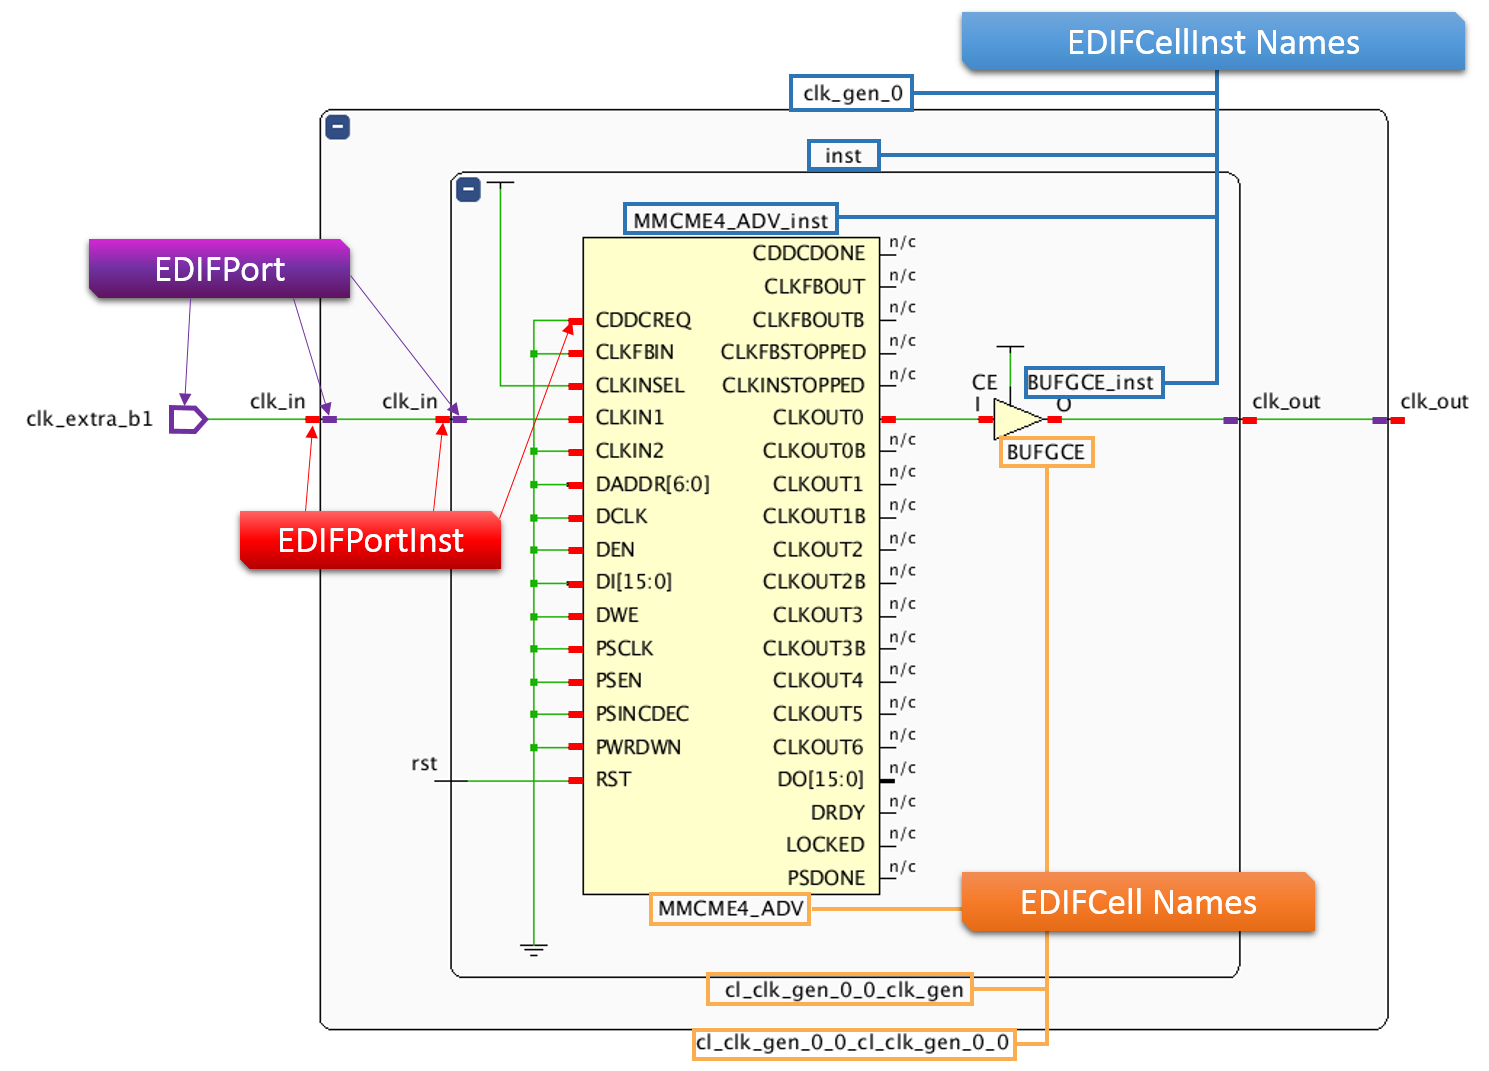
\includegraphics[width=14.0cm]{figures/edif_netlist.png}
        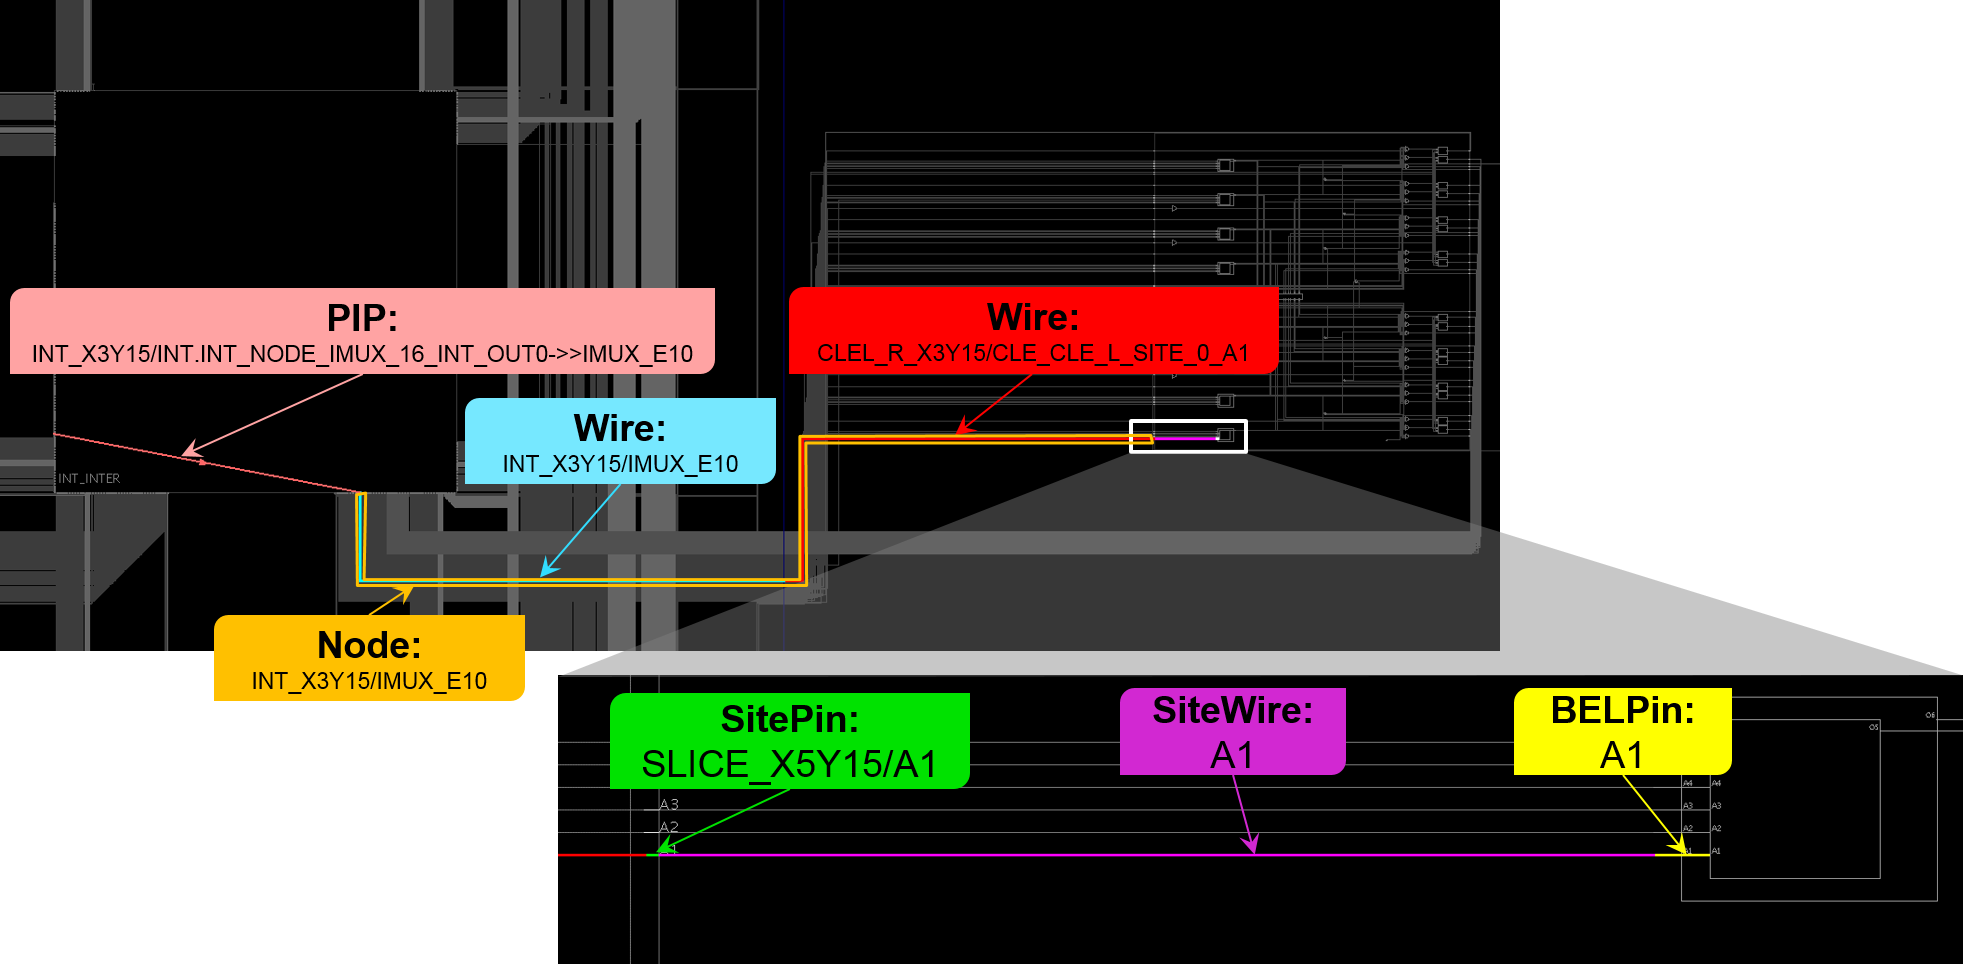
\includegraphics[width=14.0cm]{figures/routing_objects.png}
        \caption{Examples of edif netlist objects (top) and routing objects (bottom) for a Xilinx FPGA}
        \label{fig:edif_objects}
    \end{figure*}

    
    RapidWright reads in a post-synthesis design checkpoint and allows us to traverse the netlist's logical EDIFCells through various function calls. 
    For each EDIFCell object in the netlist, we create a Cell design object, which we then place onto physical device BEL object. 
    CellPins and Nets are automatically generated from EDIFHierPortInst and EDIFHierNet upon the Cell's creation from an EDIFHierCellInst. 

    These three steps correspond to our placement substages of PrePacking, Packing, and Placement, respectively.

    For a complete understanding of the RapidWright packages, please refer to the API Overview \url{https://www.rapidwright.io/docs/RapidWright_Overview.html}.


\section{Placement Implementation}

    With a basic understanding of FPGA architecture, design placement, and RapidWright, we have all the necessary pieces to implement our SA placer. 
    Here we outline in detail each substage of our implementation. 

    \begin{figure*}[t]
        \centering
        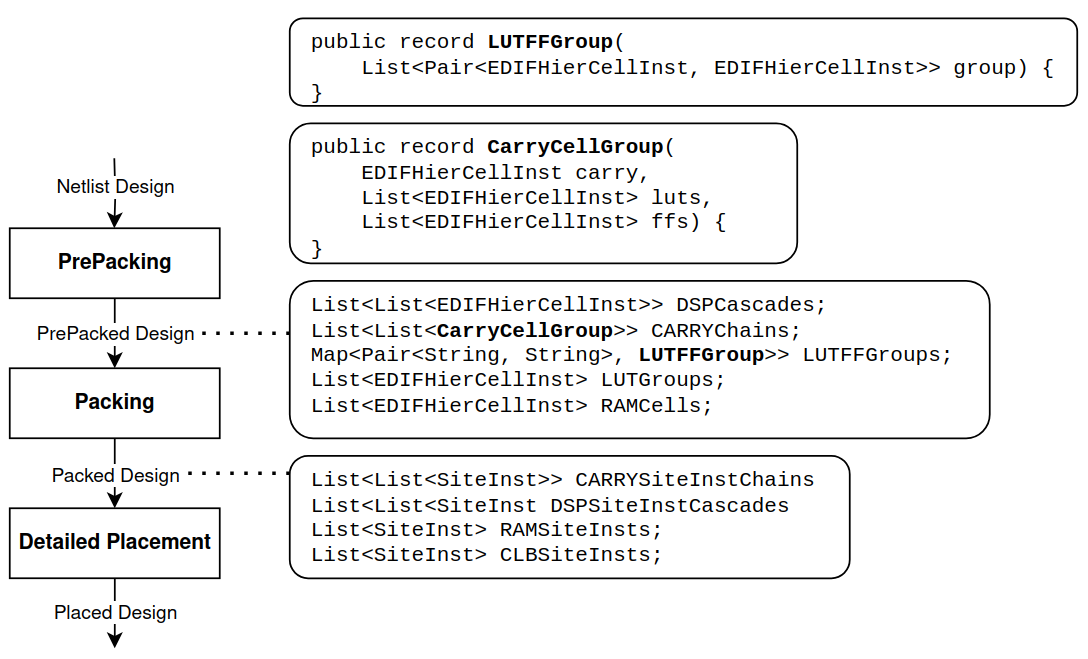
\includegraphics[width=14.0cm]{figures/substages.png}
        \caption{The data classes populated at each substage: PrepackedDesign, PackedDesign, and PlacedDesign.}
        \label{fig:substages}
    \end{figure*}

    \subsection{PrePacking}
        In the prepacking stage, we traverse the raw EDIF Netlist to identify common recurring Cell patterns. 
        We do this because there are certain desirable cell configurations that should be clustered together to exploit some proximity characteristics of the FPGA architecture. 
        There are also some cell configurations that must necessarily be placed in certain ways in relation to each other to ensure legality within the architecture constraints. 
        First, we traverse the entire EDIF netlist and identify all unique Cell types and group them together via a {\tt HashMap<String, List<EDIFHierCellInst>>}, where String is the name cell type. 
        Cell type groups can include {\tt CARRY4}, {\tt LUT1-6}, {\tt FF}, {\tt DSP48E1}, {\tt RAMB18E1}, and others. 
        We specifically look for CARRY chains, DSP cascades, and LUT-FF pairs as these patterns are common to nearly all FPGA designs.

        \subsection{CARRY Chains}
            \begin{figure}[]
                \centering
                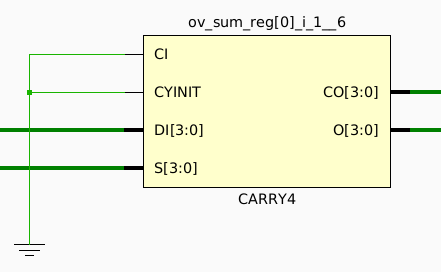
\includegraphics[width=5.0cm]{figures/carry_cell_edif.png}
                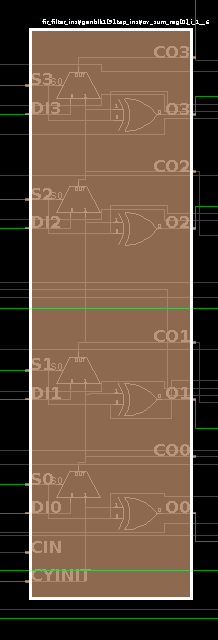
\includegraphics[width=3.0cm]{figures/carry_cell_device.png}
                \caption{
                    Left: A CARRY4 EDIFCell as seen in the Vivado netlist viewer.
                    Right: The corresponding CARRY4 Cell as seen in the device viewer.
                }
                \label{fig:carry_cell_edif}
            \end{figure}

            \begin{figure*}[t]
                \centering
                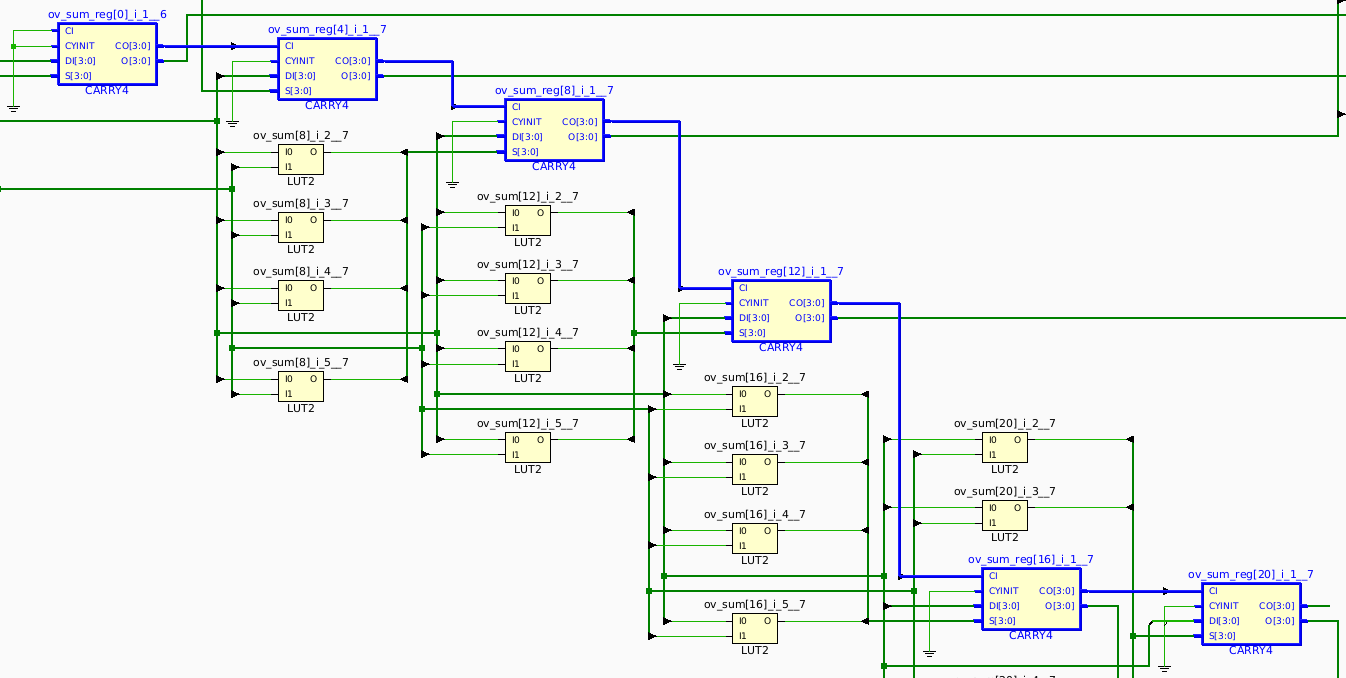
\includegraphics[width=\textwidth]{figures/carry_chain_edif.png}
                \caption{Example of a CARRY4 chain of length 6 as seen in the Vivado netlist viewer.}
                \label{fig:carry_chain_edif}
            \end{figure*}

            
            To find CARRY chains, we take the CARRY4 group and follow the below pseudocode. 

            Each SLICE Site contains one CARRY4 BEL.
            Each CLB Tile contains two SLICE Sites.
            CARRY chains span vertically across multiple SLICE Sites/Tiles. (Show picture)
            \begin{figure}
                \centering
                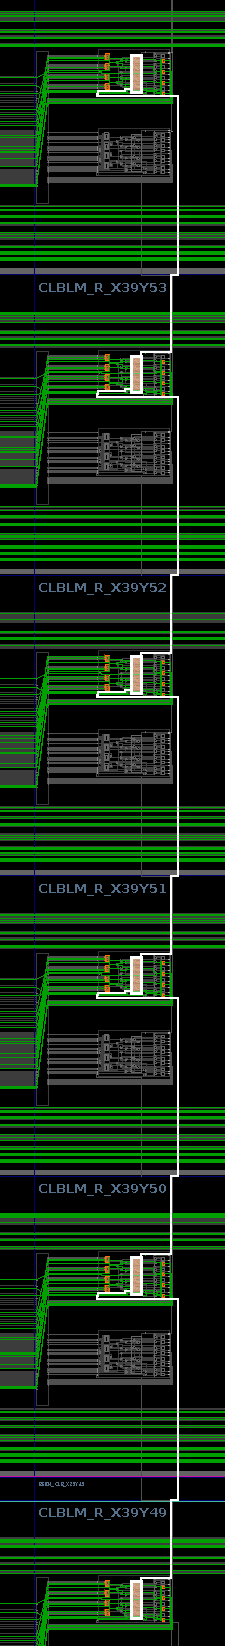
\includegraphics[width=3.0cm]{figures/carry_chain_routes.png}
                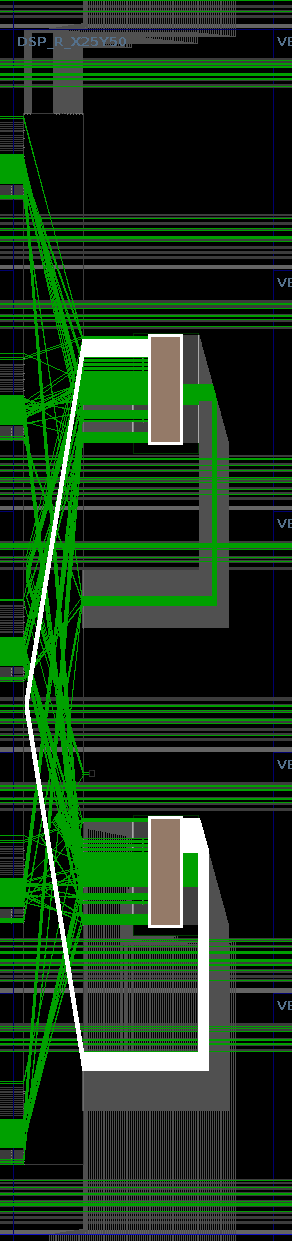
\includegraphics[width=3.0cm]{figures/dsp_cascade_routes.png}
                \caption{Left: A Carry Chain of length 6 spanning 6 Sites across 6 Tiles. On the left, the cell-only representation. Right: A DSP cascade of length 2 spanning 2 Sites across 1 Tile.}
                \label{fig:device_carry_chain_routing}
            \end{figure}
        \subsection{DSP Cascades}
            Each DSP Site contains one DSP BEL.
            Each DSP Tile contains two DSP Sites.
            DSP chains can span vertically across multiple DSP Sites/Tiles.

        \subsection{LUT-FF Pairs}
            Identify unique CE-SR net pairs. All FF cells in a Site must share the same CE and SR nets.
    \subsection{Packing}
        In the packing stage, we take the identified cell clusters and pack them into SiteInst Design objects which target the Device Site objects.
        \subsection{CLB Sites}
            Can support LUT-FF pairs, loose LUTs, loose FFs, CARRY chains.
            Each SLICE has 8 "lanes" of LUT-FFs. 4 LUT5s and 4 LUT6s. 8 FFs.
            For SLICEMs, LUT6s can be configured as shallow 32-bit LUTRAMs or "RAMS32".
    \subsection{Placement: Simulated Annealing}
        Create BEL "fields": CLB, DSP, CLB and DSP Chains, RAMs

        \subsection{Detailed Placement}

\section{Placement Results}





% \section{Analytical Placement}
%     Introduce placement with legalization methods. \\
%     Many AP approaches use a Global placement, Legalization, then Detailed placement approach. \\
%     Our SA only considers legal moves via bookkeeping structures, so it has no concept of global placement or legalization. \\
%     It is a detailed placement only approach. \\
%     \begin{itemize}
%         \item Talk about HeAP as an example.
%         \item Global Placement, Legalization, then Detailed Placement approach.
%         \item Global placement using the Bound2Bound net model from SimPL.
%         \item Legalization Step 1: \\
%             Find an area of the device that is overutilized (illegal) for twhich the blocks contained within must spread to a larger area. \\
%             To obtain this overutilized area, adjacent locations (Sites, Tiles, etc.) on the device that are occupied by more than one block (SiteInst, ModuleInst, etc.) are repeatedly clustered together, until all clusters are bordered on all sides by non-overutilized locations. \\ 
%             Then, the area (?) is expanded in both the x and y dimensions (?) until it is large enough to accommodate all blocks contained within. \\
%             Specifically, the area is expanded until its "occupance" \(O_A\) divided by its "capacity" \(C_A\) is less than a maximum "utilization factor" $\beta$, where $\beta$ is less than or equal to 1. HeAP uses 0.9.
%         \item Legalization Step 2: \\
%             Two cuts are generated: a "source cut" and a "target cut". \\
%             The source cut pertains to the blocks being placed (SiteInsts in home buffer). \\ 
%             The target cut pertains to the area into which the blocks are placed (away buffer). \\
%             The source cut splits the blocks into 2 partitions, while the target cut splits the area into 2 sub-areas, into which the blocks in each partition are spread. \\
%             Two objectives are minimized during this process: The imbalance between the number of blocks in each partition, and the difference in the utilization of each sub-area. \\
%             Utilization defined as the occupancy divided by the capacity of the sub-area. \\
%             \(U_{sub-area} = \frac{O_{sub-area}}{C_{sub-area}}\) \\
%             To generate the source cut, the cells are first sorted by their x or y location, depending on the orientation of the desired cut. \\
%             Once the cells are sorted, the source cut generation is akin to choosing a pivot in a sorted list, where all blocks to the left of the pivot are assigned to the left/bottom partition and all blocks to the right of the pivot are assigned to the right/top partition. \\
%             The target cut is an x or y cut of the area such that all blocks in each partition fit in their respective sub-areas, and such that \( | U_{sub-area_1} 
%              - U_{sub-area_2} | \) is minimized.
%     \end{itemize}





\end{document}
